\def\currentRootFolder{chapter/sensitivityStudyWithPreliminaryKatrinElossModel/statisticalPrerequisites}
\def\currentFigureFolder{\currentRootFolder/fig}
\newcommand{\elecIndex}{\mathrm{e}}

\newcommand{\Bsource}{B^j_\mathrm{S}}
\newcommand{\BsourceAvg}{B_\mathrm{S}}
\newcommand{\zSource}{z_\mathrm{S}}
\newcommand{\thetaSource}{\theta_\mathrm{S}}
\newcommand{\thetaSourceAvg}{\theta_\mathrm{S}}
\newcommand{\Esource}{E_\mathrm{S}}
\newcommand{\Usource}{U^j_\mathrm{S}}
\newcommand{\gammaSource}{\gamma_\mathrm{S}}


\newcommand{\Bps}{B_\mathrm{PS2}}
\newcommand{\Bana}{B_\mathrm{A}}
\newcommand{\Bpinch}{B_\mathrm{P}}
\newcommand{\Bmax}{B_\mathrm{max}}
\newcommand{\Bmin}{B_\mathrm{min}}

\newcommand{\thetaMax}{\theta_\mathrm{max}}
\newcommand{\Esur}{E_\mathrm{sur}}
\newcommand{\detEff}{\epsilon_\mathrm{det}}
\newcommand{\macefilterwidth}{\Delta \mathcal{E}^j(\thetaS^j)}

\newcommand{\EtransPure}{E^j_\mathrm{tr}}
\newcommand{\Etrans}{\EtransPure(qU,\Esource,\thetaSource)}
\newcommand{\thetaTransPure}{\theta^j_\mathrm{tr}}
\newcommand{\thetaTrans}{\thetaTransPure(\Esource,qU)}

\newcommand{\As}{A_\mathrm{S}}
\newcommand{\Rbg}{R_\mathrm{bg}}


\newacronym{standardmodel}{SM}{Standard Model of Particle Physics}
\newacronym{lep}{LEP}{Large Electron Positron Collider}
\newacronym{ssm}{SSM}{standard solar model}

\section{Statistical Prerequisites}
\label{sec:katrinElossStatistics}
This section develops the statistical tools used in the scope of this thesis in order to evaluate the impact of the KATRIN model on KATRIN's sensitivity to the neutrino mass. The methods are described in a general manner (and could be applied to study model uncertainties in general) and then related to the KATRIN model. Section~\ref{sec:katrinElossStatisticsCombMeasurements} presents a concept for the combination of multiple measurements in parameter inference. Section~\ref{sec:katrinElossStatisticsProfileLikelihood} introduces the profile likelihood method for the treatment of nuisance parameters. And section~\ref{sec:katrinElossStatisticsImplementation} outlines how the statistical concepts were implemented into the KaFit (see section~\ref{sec:statMethodsKaFitSSC}) software framework.

\subsection{Combination of Commissioning and Neutrino Mass Measurements}
If two measurements share a set of parameters $\paramVecShared$, but have additionally an individual set of parameters $\paramVec_1$ and $\paramVec_2$ and different sets of observations a combined likelihood is given by the product of the single likelihoods $L_1$ and $L_2$~\cite{ReviewOfParticlePhysics}
\newcommand{\paramVecSOne}{\paramVec_\mathrm{1,s}}
\newcommand{\paramVecSTwo}{\paramVec_\mathrm{2,s}}
\begin{align}
-2\ln L(\paramVecShared, \paramVec_1, \paramVec_2) &=  
-2\ln L_1(\paramVecShared, \paramVec_1)
-2\ln L_2(\paramVecShared, \paramVec_2)
\nonumber \\
&\equiv
-2\ln L_1(\paramVecSOne)
-2\ln L_2(\paramVecSTwo)
\fullstop
\end{align}
where, for ease of notation, the combined parameter vectors $\paramVec_\mathrm{s,1}\equiv(\paramVec_\mathrm{s},\paramVec_1)$ and 
$\paramVec_\mathrm{s,2}\equiv(\paramVec_\mathrm{s},\paramVec_2)$ are introduced. The first measurement could be sensitive to the neutrino mass whereas the second measurement could have been a calibration or commissioning measurement and be sensitive to parameters of the response function (see equation~\ref{eq:intSpecModelResponse}). Combining both likelihoods would incorporate the uncertainties on the parameters of the response function in the neutrino mass determination. 

For practicality, in this thesis, an approximation is applied: The calibration measurement is seen as evaluated independently and one obtains estimates $\hat{\paramVec}_\mathrm{2,s}$, and an estimated covariance matrix $\hat{V}_\mathrm{2,s}$. These can in turn be used to approximate the likelihood $L_2$. A choice that stands to reason for the approximation of $L_2$ is a multivariate normal distribution $\mathcal{N}$. For the purpose of parameter inference through the maximum likelihood method $-2\ln L_2$ needs only to be accurately approximated within the contour, that is needed to extract uncertainty intervals. The choice of a multivariate normal distribution corresponds a symmetric approximation of $-\ln L_2$ around its minimum by a second order function. The combined likelihood then reads
\begin{equation}
\begin{split}
\label{eq:penalizedLikelihood}
-2\ln L(\paramVecShared, \paramVec_1, \paramVec_2) &\approx
-2\ln L^\prime(\paramVecShared, \paramVec_1) \\ &=
\underbrace{
	\chi^2(\paramVecSOne)
	\vphantom{(\paramVecSTwo - \hat{\paramVec}_\mathrm{s,2})^{\mathsf{T}}}
}_{(1)}
+
\underbrace{
	(\paramVecShared - \hat{\paramVec}_\mathrm{s,2})^{\mathsf{T}}
	\hat{V}_\mathrm{s,2}^{-1}
	(\paramVecShared - \hat{\paramVec}_\mathrm{s,2})
}_{(2)} +\; 
\mathrm{ constants}\\ &=
\chi^2(\paramVecSOne) 
-2\ln \mathcal{N}(\paramVecSTwo, \hat{\paramVec}_\mathrm{s,2}, \hat{V}_\mathrm{s,2}^{-1}) +
\mathrm{ constants}
\end{split}
\end{equation}
Here, $(1)$ is the chi-square likelihood for a KATRIN neutrino mass measurement (see equation~\ref{eq:statMethodsKatrinChi2}). And $(2)$ resembles the negative log likelihood of the calibration measurement approximated by a multivariate normal distribution. Terms having a form like $(2)$ are also sometimes called ``pull terms'' because in the minimization of the likelihood they ``pull'' the parameters $\paramVecShared$ towards the corresponding values in $\hat{\paramVec}_\mathrm{s,2}$.

The chi-square term $(1)$ is a sum of $n$ standard normal distributed random variables. Hence, as discussed in section~\ref{sec:statMethodsKATRINLikelihood}, a likelihood only composed of the chi-square term $(1)$ offers a goodness-of-fit criteria via the the Pearson chi-square statistic. Whether the same criteria can be applied to the combined likelihood has to be investigated individually from case to case.

\paragraph{Application to the KATRIN Energy Loss Model}
With regard to the study presented in this chapter, the following identification can be made. $\paramVec_1$ comprises the parameter of a nominal four-parameter KATRIN neutrino mass fit (see section~\ref{sec:statMethodsStandardFit}). Furthermore, the commissioning/calibration measurement can be identified with the measurement of the KATRIN energy loss model $\hat{\paramVec}_\mathrm{s}=\hat{\nuisanceParamVec}_\mathrm{eloss}$, $\hat{\paramVec}_2=\hat{\nuisanceParamVec}_\mathrm{eloss+}$ and the corresponding covariance matrix $\hat{V}_\mathrm{s,2}$. The numerical values for the later three can be found in appendix~\ref{sec:appendixKatrinElossElossModelParams}.

\subsection{Nuisance Parameters and the Profile Likelihood Method}
\label{sec:katrinElossStatisticsProfileLikelihood}
\begin{figure}[t]
	\centering
	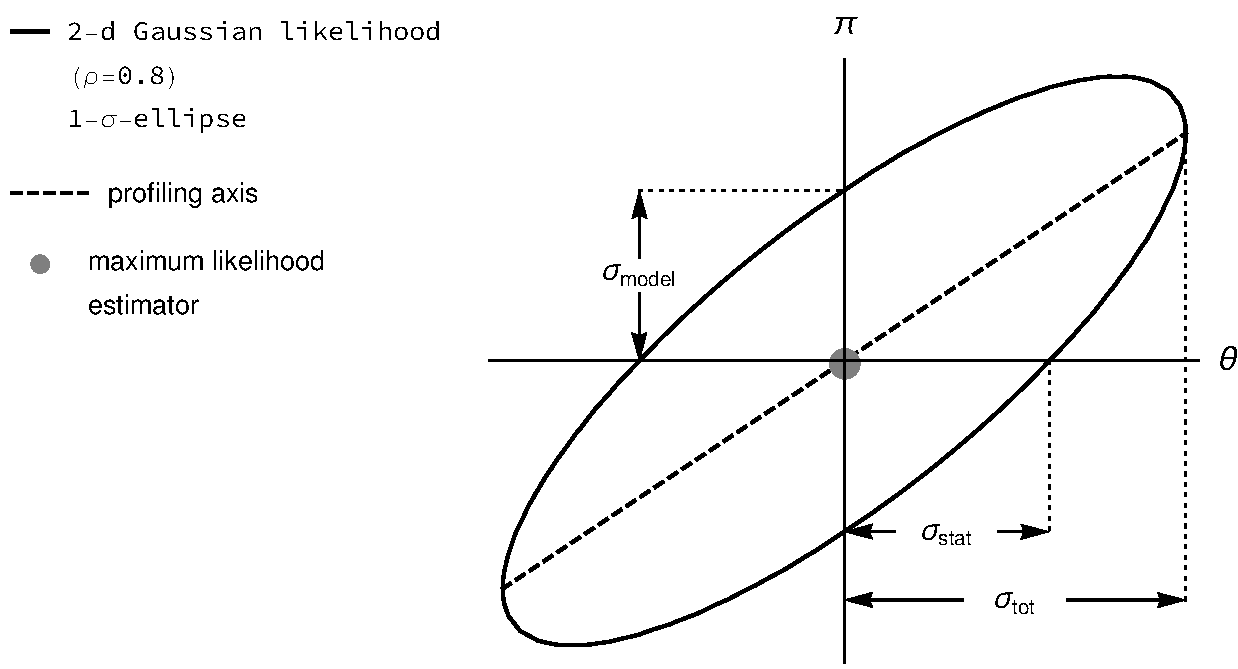
\includegraphics[width=\textwidth]{\currentFigureFolder/profileLikelihood.pdf}
	\xcaption{}{}{}
	\label{fig:katrinElossStatisticsProfileLikelihood}
\end{figure}
Apart from the  parameters of interest $\paramVec$ (usually the squared neutrino mass), the KATRIN likelihood depends on further so-called nuisance parameters $\nuisanceParamVec$. The dimensionality may pose difficulties when deriving a confidence region for the combined parameter set. Furthermore, as indicated by the naming conventions, the dimensions of the nuisance parameters in the confidence region are not of interest. Hence, in order to derive a confidence interval with just one dimension, a test statistic, similar to the one in equation~\ref{eq:statMethodsLikelihoodRatio}, but that solely depending on the parameters of interest, has to be found. The following paragraph outlines, how a corresponding test statistic can be constructed using the profile likelihood method.

A corresponding derivation may start with the definition of the profile likelihood: The profile likelihood only depends on the parameters of interest $\paramVec$ and not on the nuisance parameters $\nuisanceParamVec$. Its values correspond the likelihood values evaluated at $\paramVec$ in the dimensions of the parameters of interest and maximized in the dimensions of the nuisance parameters~\cite{ReviewOfParticlePhysics}
\begin{equation}
\profLikelihood(\paramVec) = 
L(\paramVec, \hat{\hat{\nuisanceParamVec}}(\paramVec))
\comma
\end{equation}
where the double-hat indicates the maximization respectively the profiling. Also, the profile likelihood ratio can be defined~\cite{ReviewOfParticlePhysics}
\begin{equation}
\label{eq:statMethodsProfileLikelihoodRatio}
\lambda_\mathrm{p}(\paramVec) = 
\frac{\profLikelihood(\paramVec)}{\profLikelihood(\hat{\paramVec})}
\fullstop
\end{equation}
According to Wilks’ theorem~\cite{wilks1938}, the distribution of $-2\ln\lambda_\mathrm{p}(\hat{\paramVec})$, where $\hat{\paramVec}$ is the \gls{mle} (see section~\ref{sec:statMethodsMLE}), approaches a chi-square distribution in the limit of a large data sample size, independently of the values of the nuisance parameters $\nuisanceParamVec$~\cite{ReviewOfParticlePhysics}. Hence, the profile likelihood ratio offers a test statistic, from which a confidence interval for the parameters of interest can be derived. However, it should be noted that whether the limit of a large sample size is given has to be investigated individually from case to case.

\subsection{Extension of the KaFit Software Framework}
\label{sec:katrinElossStatisticsImplementation}
The likelihood $L(\paramVec)$ can be multiplied by a function $g(\paramVec)$
\begin{equation}
\label{eq:likelihoodExtension}
-2\ln L^\prime(\paramVec) = -2\ln L(\paramVec) -2\ln g(\paramVec)
\fullstop
\end{equation}
This procedure may have different interpretations and usage scenarios. E.g. a comparison with \eqref{eq:posterior} shows, if $g$ is a prior probability distribution, $L^\prime$ becomes a non-normalized posterior distribution that can be used in a Bayesian analysis. A further interpretation is given in section \ref{sec:combinationOfMeasurements}.
\label{sec:combinationOfMeasurements}

KaFit allowed to choose $g$ in \ref{eq:likelihoodExtension} as a product of one-dimensional Gaussian distributions. Within this thesis the software was extended to allow products of other functions. Three function types were explicitly made available through a configuration file.
\begin{enumerate}
	\item A reimplementation of a one-dimensional Gaussian distribution: The reimplementation was necessary to conveniently enable the combination of function types.
	\item A multivariate Gaussian distribution: This enables the treatment of uncertainties quantified by calibration or monitor measurements as described in section \ref{sec:combinationOfMeasurements}. It can also be used as a prior distribution in a Bayesian analysis. Particularly, correlations can be respected.
	\item A one-dimensional probability density, that is constant in the square root of a parameter, if it is positive and 0 otherwise:
	\begin{equation}
		g(\theta) =
		\begin{cases}
		0 &\text{ if } \theta \leq 0 \\
		\text{constant} \cdot \frac{1}{\sqrt{\theta}} &\text{ if } \theta > 0
		\end{cases}
		\fullstop
	\end{equation}
	 This can be used as a uniform prior on the neutrino mass ($\theta=m_\nu^2$). Formerly, it was only possible to use a uniform prior on the squared neutrino mass. A derivation of the form of $g$ can be found in appendix \ref{sec:appStatisticPriorOnNu2}.
\end{enumerate}
An example on how to configure KaFit using the new feature is given in appendix \todo{Add appendix}.
